\documentclass[10pt]{article}
\usepackage[margin=0.72in]{geometry}
\usepackage{amsmath,booktabs,longtable,array,graphicx,xcolor,hyperref,seqsplit}
\hypersetup{colorlinks=true,linkcolor=blue,urlcolor=blue}
\newcommand{\pass}{\textcolor{green!45!black}{PASS}}
\newcommand{\fail}{\textcolor{red!70!black}{FAIL}}
\title{Data-volume calibration for resolving the three-mode slow relaxation band}
\author{Frozen synthetic-covariance audit}
\date{9 September 2026}
\begin{document}
\maketitle
\begin{abstract}
We calibrate how many independent trajectories are required to separate two nearby real relaxation rates using the empirical cross-lag covariance of the controlled three-mode data. The complete frozen grid comprises 336 cells and 168,000 nonlinear-fit replicates. The target spacing $\Delta=0.20$ fails for both driven and equilibrium covariance at every tested stream count through $N=2048$, for both fit windows and both amplitude constraints. The predeclared Part-2 gate is therefore closed and no additional physical trajectory simulation is launched. The result is a quantitative non-resolution bound, not evidence that the physical slow band is absent.
\end{abstract}
\section{Question and frozen protocol}
The synthetic truth is
\[C(t)=0.6e^{-0.90t}+0.4e^{(-0.90-\Delta)t},\]
with $\Delta\in\{0.05,0.10,0.15,0.20,0.30,0.40,0.60\}$ and $N\in\{64,128,256,512,1024,2048\}$. Noise preserves the full empirical cross-lag covariance of the saved $I_2$ correlation curves and scales as $\sqrt{64/N}$. We use 500 deterministic replicates per case--$N$--$\Delta$--window--constraint cell.
Real sums of one to four exponentials are selected sequentially by $\Delta\mathrm{AIC}\leq-10$. A cell resolves the two rates only if at least 90\% of successful fits select $m\geq2$ and both median matched-rate errors are at most $\max(0.05,\Delta/4)$. The fixed window is $[0.20,4.00]$; the extended window follows the frozen contiguous $C/\mathrm{SE}\geq3$ rule. No rule was changed after output existed.
\section{Primary result: the Part-2 gate is closed}
None of the 48 cells at the target spacing $\Delta=0.20$ passes. Consequently there is no common tested $N\leq2048$, window, and amplitude rule that resolves the target in both bath cases. Under the frozen protocol, Part 2 is forbidden.
\begin{figure}[ht]\centering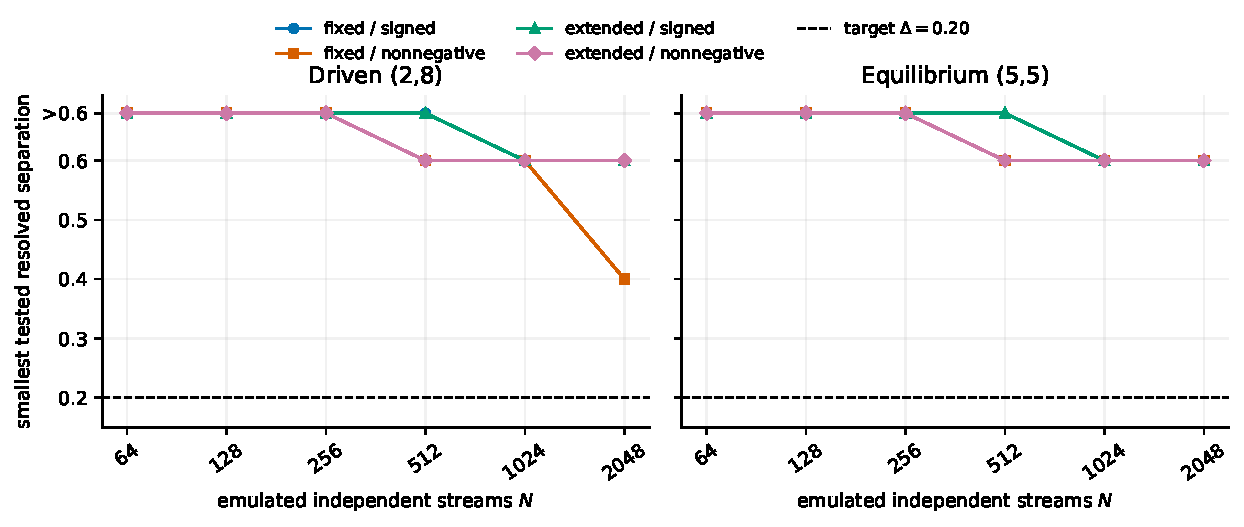
\includegraphics[width=.98\linewidth]{../figures/resolution_curves.pdf}\caption{Smallest tested separation satisfying the complete resolution rule. Values marked $>0.6$ mean no tested separation passed. The dashed line is the target $\Delta=0.20$.}\end{figure}
\begin{table}[ht]\centering\small\begin{tabular}{lllrr}\toprule Case & Window & amplitudes & smallest resolved at $N=2048$ & resolved cells\\\midrule
Driven (2,8) & fixed & signed & 0.60 & 1 \\
Driven (2,8) & fixed & nonnegative & 0.40 & 2 \\
Driven (2,8) & extended & signed & 0.60 & 1 \\
Driven (2,8) & extended & nonnegative & 0.60 & 1 \\
Equilibrium (5,5) & fixed & signed & 0.60 & 1 \\
Equilibrium (5,5) & fixed & nonnegative & 0.60 & 1 \\
Equilibrium (5,5) & extended & signed & 0.60 & 1 \\
Equilibrium (5,5) & extended & nonnegative & 0.60 & 1 \\
\bottomrule\end{tabular}\caption{Observed resolution at the largest tested stream count.}\end{table}\clearpage
\section{Why increasing \texorpdfstring{$N$}{N} did not resolve \texorpdfstring{$\Delta=0.20$}{Delta=0.20}}
The probability of selecting multiple exponentials approaches one, but the matched rate errors remain well above the 0.05 tolerance. Simultaneously, the original numerical-identifiability fraction generally decreases. Model-order selection alone is therefore not evidence that the two physical rates have been recovered.
\begin{figure}[ht]\centering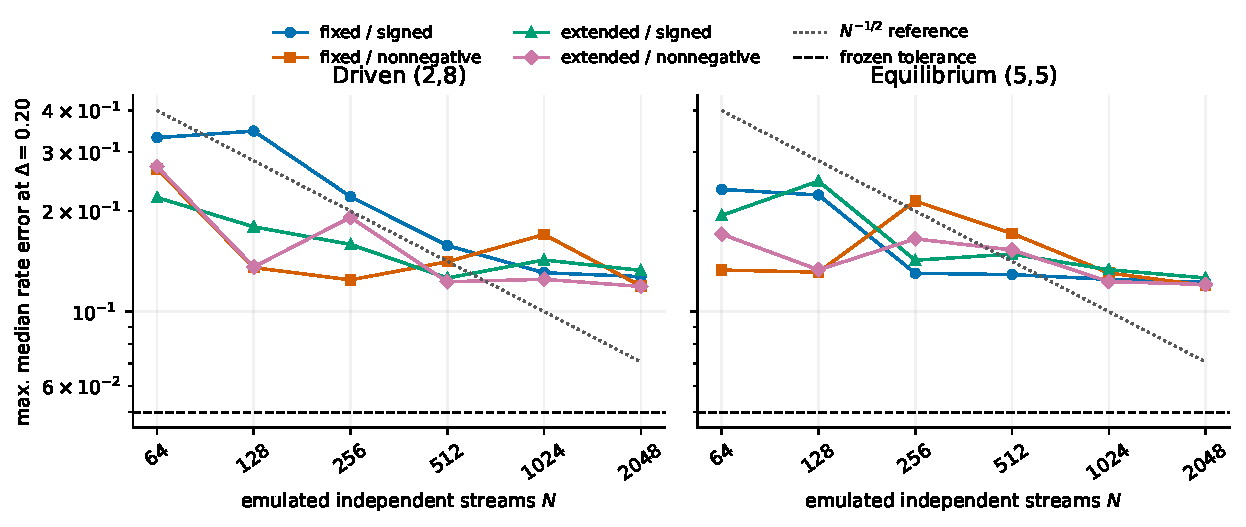
\includegraphics[width=.98\linewidth]{../figures/delta020_error_scaling.pdf}\caption{Maximum of the two median matched-rate errors at $\Delta=0.20$. The dotted $N^{-1/2}$ curve is a slope reference, not a fit; the dashed line is the frozen tolerance.}\end{figure}
\begin{figure}[ht]\centering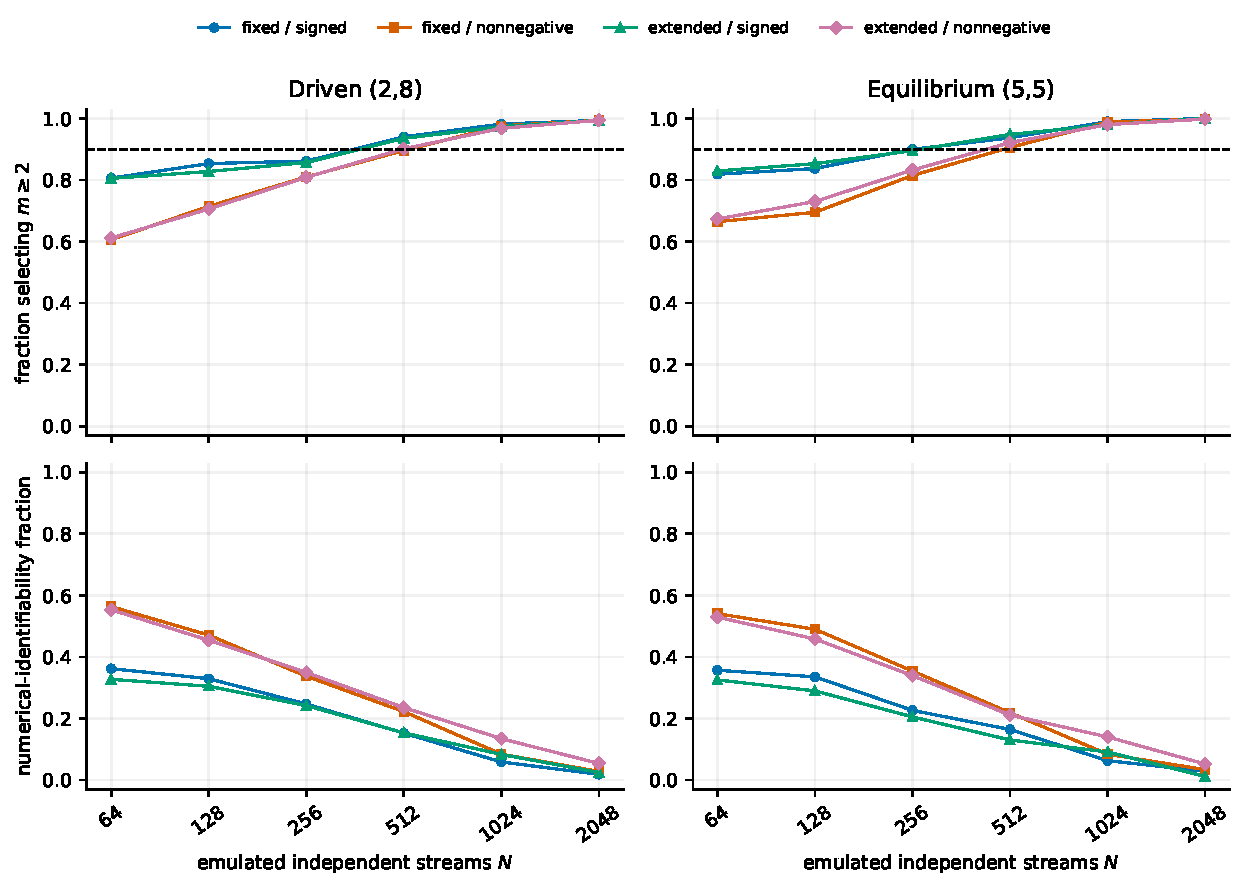
\includegraphics[width=.98\linewidth]{../figures/delta020_selection_identifiability.pdf}\caption{At $\Delta=0.20$, selection of $m\geq2$ becomes frequent while numerical identifiability deteriorates.}\end{figure}\clearpage
\section{All target-spacing summaries}
\scriptsize\begin{longtable}{llrlrrrrr}\toprule Case & Window & amplitudes & $N$ & $P(m\geq2)$ & error slow & error fast & num.-ID & pass\\\midrule\endhead
Driven (2,8) & extended & nonnegative & 64 & 0.612 & 0.272 & 0.125 & 0.553 & no \\
Driven (2,8) & extended & nonnegative & 128 & 0.706 & 0.136 & 0.126 & 0.454 & no \\
Driven (2,8) & extended & nonnegative & 256 & 0.809 & 0.192 & 0.125 & 0.350 & no \\
Driven (2,8) & extended & nonnegative & 512 & 0.901 & 0.076 & 0.123 & 0.235 & no \\
Driven (2,8) & extended & nonnegative & 1024 & 0.968 & 0.072 & 0.125 & 0.135 & no \\
Driven (2,8) & extended & nonnegative & 2048 & 0.994 & 0.065 & 0.119 & 0.054 & no \\
Driven (2,8) & extended & signed & 64 & 0.805 & 0.186 & 0.220 & 0.327 & no \\
Driven (2,8) & extended & signed & 128 & 0.828 & 0.148 & 0.179 & 0.305 & no \\
Driven (2,8) & extended & signed & 256 & 0.857 & 0.159 & 0.159 & 0.242 & no \\
Driven (2,8) & extended & signed & 512 & 0.935 & 0.088 & 0.126 & 0.154 & no \\
Driven (2,8) & extended & signed & 1024 & 0.974 & 0.070 & 0.143 & 0.083 & no \\
Driven (2,8) & extended & signed & 2048 & 0.994 & 0.066 & 0.133 & 0.025 & no \\
Driven (2,8) & fixed & nonnegative & 64 & 0.606 & 0.268 & 0.128 & 0.564 & no \\
Driven (2,8) & fixed & nonnegative & 128 & 0.714 & 0.135 & 0.128 & 0.471 & no \\
Driven (2,8) & fixed & nonnegative & 256 & 0.810 & 0.121 & 0.124 & 0.337 & no \\
Driven (2,8) & fixed & nonnegative & 512 & 0.896 & 0.141 & 0.123 & 0.222 & no \\
Driven (2,8) & fixed & nonnegative & 1024 & 0.976 & 0.170 & 0.123 & 0.084 & no \\
Driven (2,8) & fixed & nonnegative & 2048 & 0.994 & 0.085 & 0.119 & 0.028 & no \\
Driven (2,8) & fixed & signed & 64 & 0.806 & 0.144 & 0.332 & 0.362 & no \\
Driven (2,8) & fixed & signed & 128 & 0.853 & 0.101 & 0.347 & 0.329 & no \\
Driven (2,8) & fixed & signed & 256 & 0.861 & 0.096 & 0.221 & 0.247 & no \\
Driven (2,8) & fixed & signed & 512 & 0.940 & 0.075 & 0.158 & 0.153 & no \\
Driven (2,8) & fixed & signed & 1024 & 0.982 & 0.072 & 0.131 & 0.059 & no \\
Driven (2,8) & fixed & signed & 2048 & 0.994 & 0.067 & 0.127 & 0.019 & no \\
Equilibrium (5,5) & extended & nonnegative & 64 & 0.673 & 0.171 & 0.132 & 0.529 & no \\
Equilibrium (5,5) & extended & nonnegative & 128 & 0.730 & 0.083 & 0.133 & 0.458 & no \\
Equilibrium (5,5) & extended & nonnegative & 256 & 0.832 & 0.165 & 0.127 & 0.339 & no \\
Equilibrium (5,5) & extended & nonnegative & 512 & 0.922 & 0.153 & 0.126 & 0.211 & no \\
Equilibrium (5,5) & extended & nonnegative & 1024 & 0.980 & 0.071 & 0.123 & 0.140 & no \\
Equilibrium (5,5) & extended & nonnegative & 2048 & 0.998 & 0.067 & 0.121 & 0.052 & no \\
Equilibrium (5,5) & extended & signed & 64 & 0.829 & 0.194 & 0.162 & 0.325 & no \\
Equilibrium (5,5) & extended & signed & 128 & 0.853 & 0.089 & 0.246 & 0.290 & no \\
Equilibrium (5,5) & extended & signed & 256 & 0.895 & 0.129 & 0.143 & 0.205 & no \\
Equilibrium (5,5) & extended & signed & 512 & 0.948 & 0.149 & 0.126 & 0.130 & no \\
Equilibrium (5,5) & extended & signed & 1024 & 0.980 & 0.069 & 0.134 & 0.091 & no \\
Equilibrium (5,5) & extended & signed & 2048 & 1.000 & 0.065 & 0.126 & 0.012 & no \\
Equilibrium (5,5) & fixed & nonnegative & 64 & 0.665 & 0.123 & 0.133 & 0.541 & no \\
Equilibrium (5,5) & fixed & nonnegative & 128 & 0.695 & 0.078 & 0.131 & 0.490 & no \\
Equilibrium (5,5) & fixed & nonnegative & 256 & 0.815 & 0.214 & 0.126 & 0.354 & no \\
Equilibrium (5,5) & fixed & nonnegative & 512 & 0.906 & 0.171 & 0.124 & 0.219 & no \\
Equilibrium (5,5) & fixed & nonnegative & 1024 & 0.988 & 0.130 & 0.123 & 0.084 & no \\
Equilibrium (5,5) & fixed & nonnegative & 2048 & 0.998 & 0.081 & 0.120 & 0.034 & no \\
Equilibrium (5,5) & fixed & signed & 64 & 0.819 & 0.118 & 0.232 & 0.357 & no \\
Equilibrium (5,5) & fixed & signed & 128 & 0.837 & 0.077 & 0.223 & 0.335 & no \\
Equilibrium (5,5) & fixed & signed & 256 & 0.900 & 0.091 & 0.130 & 0.226 & no \\
Equilibrium (5,5) & fixed & signed & 512 & 0.937 & 0.074 & 0.129 & 0.164 & no \\
Equilibrium (5,5) & fixed & signed & 1024 & 0.990 & 0.071 & 0.125 & 0.063 & no \\
Equilibrium (5,5) & fixed & signed & 2048 & 1.000 & 0.064 & 0.122 & 0.029 & no \\
\bottomrule\end{longtable}\normalsize
\section{Scaling, saturation, and descriptive extrapolation}
For each case and rule, a descriptive power law was fit to the maximum median error over $N\geq256$. Seven of eight curves meet the frozen saturation rule: the target remains unresolved at $N=2048$ and the error decreases by less than 10\% from $N=1024$ to 2048. Exponents are much shallower than the independent-stream benchmark $-1/2$. Extrapolated $N$ values do not include the separate 90\% model-selection requirement and cannot authorize production.
\small\begin{longtable}{lllrrrr}\toprule Case & Window & amplitudes & exponent & implied $N$ & reduction & saturated\\\midrule\endhead
Driven (2,8) & fixed & signed & -0.265 & 51659 & 2.6\% & yes \\
Driven (2,8) & fixed & nonnegative & 0.009 & $\infty$ & 29.9\% & no \\
Driven (2,8) & extended & signed & -0.060 & 22365519689 & 6.9\% & yes \\
Driven (2,8) & extended & nonnegative & -0.204 & 100666 & 4.8\% & yes \\
Equilibrium (5,5) & fixed & signed & -0.031 & 4744167290403765 & 2.0\% & yes \\
Equilibrium (5,5) & fixed & nonnegative & -0.291 & 35137 & 8.2\% & yes \\
Equilibrium (5,5) & extended & signed & -0.068 & 1893455711 & 5.5\% & yes \\
Equilibrium (5,5) & extended & nonnegative & -0.168 & 323382 & 2.1\% & yes \\
\bottomrule\end{longtable}\normalsize
\section{Audit and reproducibility}
The integrity audit is \pass. It reconstructs all 336 summaries from the 168,000 raw rows, verifies exactly 500 replicate indices in every cell, reproduces the Part-2 gate, and verifies the source and both input hashes.
\begin{verbatim}
python3 experiments/slow_band_resolution_scaling_2026-09-07/run_scaling.py
  --output experiments/slow_band_resolution_scaling_2026-09-07/part1_analysis
  --replicates 500 --workers 8
\end{verbatim}
Master seed: 2026091201. Runtime: 27.55 hours. Analysis source SHA-256: \texttt{\seqsplit{b2ad9a90fc9ecfd2799c9b778dff3d7194c28faca224da70f20f5db022dce1d4}}.
\begin{itemize}
\item Driven input SHA-256: \texttt{\seqsplit{9a878a637bd7475ab0f05ea0b7991276f4de1fd53f152c274530b7f99a984a47}}.
\item Equilibrium input SHA-256: \texttt{\seqsplit{f7f97e860d75414b3999d656cf585dea9d402fafe7cc1a99a22321e9963c3d45}}.
\item Previous fitting pipeline SHA-256: \texttt{\seqsplit{ada94924e17f762519a973b28712a3af57ab6f9d1987183a2459c830587d94cb}}.
\end{itemize}
All raw replicates, cell summaries, task seeds, resolution curves, extrapolation diagnostics, hashes, and the frozen protocol accompany this report.
\section{Claim boundary}
The result supports only the following statement: under the empirical covariance and frozen fitting protocol, a separation of 0.20 is not recoverable with up to 2048 emulated independent streams. It does not establish that the physical slow band is absent, and it does not justify quoting a unique spectral gap. No real-data Part-2 simulation was run because its predeclared gate failed.
\end{document}
